\documentclass{report}
\usepackage[tmargin=2cm, rmargin=1in, lmargin=1in,margin=0.85in,bmargin=2cm,footskip=.2in]{geometry}
\usepackage{amsmath,amsfonts,amsthm,amssymb,mathtools}
\usepackage{enumitem}
\usepackage[]{mdframed}
\usepackage{tikz}
\usepackage{listings}
\usepackage{graphicx}

\graphicspath{ {figures/} }



\definecolor{codegreen}{rgb}{0,0.6,0}
\definecolor{codegray}{rgb}{0.5,0.5,0.5}
\definecolor{codepurple}{rgb}{0.58,0,0.82}
\definecolor{backcolour}{rgb}{0.95,0.95,0.92}

\lstdefinestyle{c_style}{
    language=C,
    backgroundcolor=\color{backcolour},   
    commentstyle=\color{codegreen},
    keywordstyle=\color{magenta},
    numberstyle=\tiny\color{codegray},
    stringstyle=\color{codepurple},
    basicstyle=\ttfamily\footnotesize,
    breakatwhitespace=false,         
    breaklines=true,                 
    captionpos=b,                    
    keepspaces=true,                 
    numbers=left,                    
    numbersep=5pt,                  
    showspaces=false,                
    showstringspaces=false,
    showtabs=false,                  
    tabsize=2
}

\lstdefinestyle{asm_style}{
    language=asm,
    backgroundcolor=\color{backcolour},   
    commentstyle=\color{codegreen},
    keywordstyle=\color{magenta},
    numberstyle=\tiny\color{codegray},
    stringstyle=\color{codepurple},
    basicstyle=\ttfamily\footnotesize,
    breakatwhitespace=false,         
    breaklines=true,                 
    captionpos=b,                    
    keepspaces=true,                 
    numbers=left,                    
    numbersep=5pt,                  
    showspaces=false,                
    showstringspaces=false,
    showtabs=false,                  
    tabsize=2
}




\title{\Huge{CSE 120}\\Day 9 Notes}
\author{\huge{Elijah Hantman}}
\date{}

\begin{document}
\maketitle
\newpage

\begin{description}
    \item Recap Vanilla pipeline
        \begin{figure}[h]
            \centering
            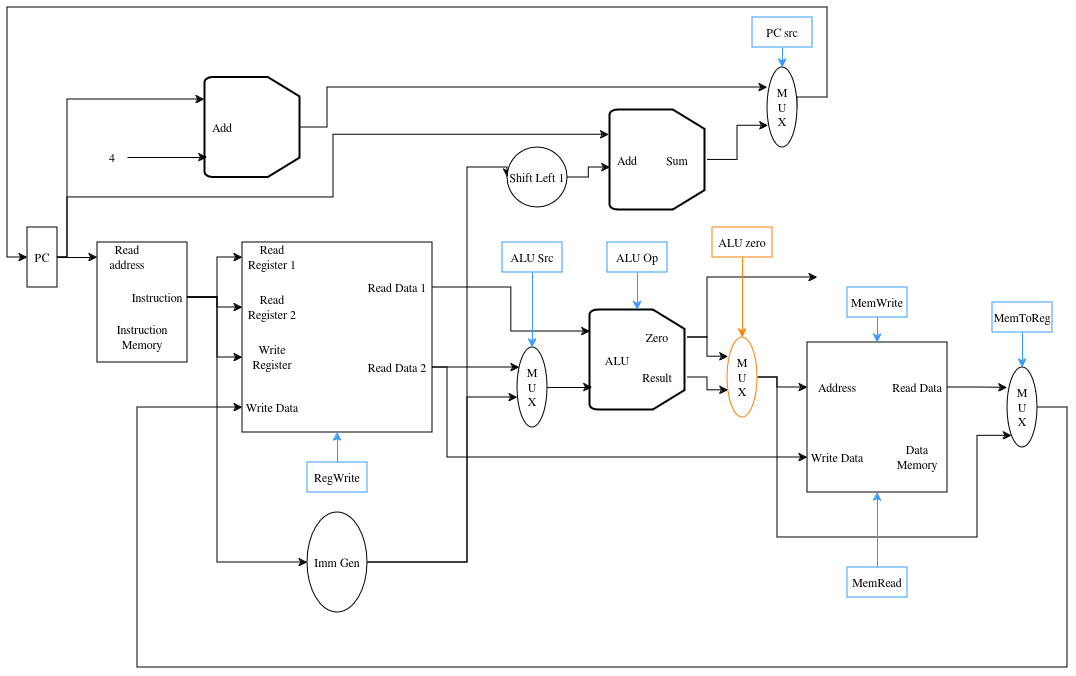
\includegraphics[scale=0.45]{modifiedDatapath}
        \end{figure}
        Five stages with pipelining between each stage.
    \item Data Hazards
        \begin{itemize}
            \item One instruction has a source operand that is
                the result of a previous instruction in the
                pipeline.
        \end{itemize}
    \item Control Hazards
        \begin{itemize}
            \item Execution depends on a branch instruction.
            \item Becomes worse with deeper pipelines, ie:
                k is large.
        \end{itemize}
        \begin{mdframed}
            Creates a tradeoff. Deep pipelines can increase
            clock frequency, however deep pipelines can
            run into many control hazards which causes massive
            slow down.
        \end{mdframed}
    \item Data dependency
        \begin{itemize}
            \item True Dependence, can cause RAW hazard
                \begin{lstlisting}[language={[x86asm]Assembler}]
                add t0, t1, t2
                sub t3, t4, t0
                \end{lstlisting}
            \item Output Dependence, can cause WAW hazard
                \begin{lstlisting}[language={[x86asm]Assembler}]
                    add t0, t1, t2
                    sub t0, t4, t5
                \end{lstlisting}
            \item Anti Dependence, can cause WAR hazard
                \begin{lstlisting}[language={[x86asm]Assembler}]
                    add t0, t1, t2
                    sub t1, t3, t5
                \end{lstlisting}

        \end{itemize}

    \item RAW example
        \begin{mdframed}
            5 Instructions fed into the pipeline.
            \begin{lstlisting}[language={[x86asm]Assembler}]
    sub x2, x1, x3  ;start of dependence
    and x12, x2, x5 ;Hazard starts
    or x13, x6, x2
    add x14, x2, x2 ;Hazard ends, depends on when writes happen in cycle
    sd x15, 100(x2) ;first instruction is readable
            \end{lstlisting}

            Fast register? A fast register will force writes
            to happen earlier in the clock cycle than the read,
            so it can be written to and read in the same cycle.

            If a register is not fast when the read happens
            is undefined.
        \end{mdframed}
    \item Solutions for RAW hazards
        \begin{itemize}
            \item One way is to stall the pipeline.
                \begin{itemize}
                    \item First you detect the hazard
                    \item pause execution
                \end{itemize}
            \item We can delay the instruction in the sequence?
                \begin{itemize}
                    \item NOP can delay instructions
                    \item Advantage: simplifies hardware
                        massively to not need to detect
                        hazards.
                    \item Disadvantage: programs are pipeline
                        specific. The number of NOPs are 
                        dependent on the pipeline.
                \end{itemize}
            \item Hardware automatically inserts NOPS
                \begin{itemize}
                    \item Advantage: correct for all programs
                    \item Disadvantage: may miss some optimization
                        opportunities
                \end{itemize}

            \item Most modern machines use hardware NOPS
        \end{itemize}
    \item Manual NOP Insertion
        \begin{mdframed}
            One common NOP is
            \begin{lstlisting}[language={[x86asm]Assembler}]
            addi x0, x0, 0
            ;or you can use
            00000000000000 ;this is an instruction with 0s in all 32 bits
            \end{lstlisting}
            
            By inserting NOPS we can prevent hazards.
            NOPS also tend to degrade performance, because they
            still force alignment to a clock cycle divisible by
            k, which will affect CPI.
        \end{mdframed}

    \item Data Forwarding
        \begin{itemize}
            \item What if we can detect RAW conflict?
            \item We can generate the most recent value in the
                pipeline, then we can backpropagate it to
                the preceeding stage.

            \item When should we forward values to avoid RAW?
            \item Figure out when the RAW will take place.
            \item You can use a Mux alongside a dirty bit

                Set the bit when you have a value that needs
                to be forwarded, unset the bit when it gets
                written back.

                Maybe multiple bits to keep track of which
                registers are "dirty"

            \item forward unit that sits between ALU and
                previous pipeline registers to decide whether
                to data forward or not.

                All thats needed is to read the write signals
                as well and you can simple compare whether the
                write signals match, and if so you use data
                forwarding.
            \item When forwarding you have to make sure it
                only forwards from the most recent dependence.
                
            \item Forward pipelining can get complicated
                super fast
        \end{itemize}
    \item Forwarding for L/S
        \begin{itemize}
            \item Consider:
                \begin{lstlisting}[language={[x86asm]Assembler}]
            ld x10, 40(x1)
            sd x10, 20(x3)
                \end{lstlisting}
            \item Can forwarding save from unwanted NOPS?
            \item The address is avalible in time to write
                to write to memory, however we need to manage
                forwarding into Data memory stage.

            \item If a bottleneck stage, data forwarding can
                negatively affect the clock speed. 
        \end{itemize}

    \item Hazard Detection for stalling the Pipeline
        \begin{mdframed}
            Forwarding can't always save the day.
            \begin{lstlisting}[language={[x86asm]Assembler}]
            ld x2, 20(x1)
            and x4, x2, x5
            \end{lstlisting}

            If you don't get the value in time to use it
            data forwarding is physically unable to help.

            The above scenario can only e solved via stalling.
        \end{mdframed}
        \begin{mdframed}
            Hazard detection condition for compulsory stall
            check textbook
        \end{mdframed}

        \begin{mdframed}
            How do we introduce a stall?

            We insert a Nop directly into the pipeline
            and delay the previous stages by one.

            \vspace{10}

            How do we generate bubbles?

            We add a control to the PC and IF/ID pipeline registers.
            The control lines prevent the PC from advancing, and the
            IF/ID registers from being written to.

            It will also pass on a zero instruction to the stages
            after the Decode. This prevents smashing memory or
            registers.
        \end{mdframed}

    

\end{description}


\end{document}
